\documentclass[preprint,12pt,a4paper]{elsarticle}

\usepackage{graphicx}
\usepackage{amsmath,amssymb}
\usepackage{booktabs}
\usepackage{multirow}
\usepackage{array}
\usepackage[hidelinks]{hyperref}
\usepackage{lineno}

\graphicspath{{figures/}}
\journal{Journal of Systems Architecture}

\begin{document}

\begin{frontmatter}

\title{Where Should the Long Wires Go? Total-Wire, Longest-Wire and Performance Trade-offs in Radix-4 On-Chip Networks}

\author{Rahul Ray}
\ead{rahulrayconnect@gmail.com}
\address{Department of Computer Science and Engineering, Assam University, Silchar 788011, India (B.Tech. 2023)}

\begin{abstract}
A 2D mesh leaves $4n$ router ports unused on the boundary of an $n\times n$
grid. Tori spend them on wraparound links; other designs fold links back
along the edges to save wire. Which choice is best depends on two different
wire costs: total wire, which sets area and link energy, and the longest
wire, which limits the clock. We formulate the use of these spare ports as a
matching problem that contains the mesh, the torus and edge-folded designs,
and search it under explicit total-wire and longest-wire constraints.
Designs are evaluated with a cycle-level simulator validated against
BookSim~2, seven dependency-driven PARSEC traces, and DSENT area, energy and
timing models at 22~nm. On an $8\times 8$ network, a searched layout whose
extra links are at most five tiles long is the fastest evaluated design at a
fixed 2~GHz clock, with 17\% lower runtime and 23\% lower energy-delay
product than a mesh under compressed traffic, using 20\% less wire than a
torus. When the longest wire limits the clock, the folded torus is best, and
edge-folded designs that keep full-length wraparounds lose to the mesh.
\end{abstract}

\begin{keyword}
network-on-chip \sep topology \sep wire length \sep deadlock-free routing \sep simulated annealing \sep reinforcement learning \sep DSENT \sep BookSim
\end{keyword}

\end{frontmatter}

\linenumbers

% ===========================================================================
\section{Introduction}
\label{sec:intro}

Most many-core chips still connect their tiles with a 2D mesh. It maps
directly onto the floorplan, every link is one tile long, and every router
has the same five ports (four neighbours and the local core). Its weakness
is distance: a packet may need $2(n-1)$ hops on an $n\times n$ grid. The
classic remedy is to add long links. A torus closes every row and column
into a ring; express links, flattened butterflies and low-diameter graphs
go further \cite{dally2004principles,slimnoc,shg}.

Long links are paid for twice. Their \emph{total} length sets wire area,
repeater area and link energy. Their \emph{maximum} length sets how fast
the network can be clocked, because a wire that does not fit in one cycle
either lowers the clock or must be pipelined. Recent chiplet work makes
the second cost explicit: Kite classifies interposer topologies by their
longest link and shows that long-link topologies lose much of their hop
advantage once each runs at the clock its longest wire allows
\cite{kite}. NetSmith automates the same design problem with mixed-integer
programming under link-length limits \cite{netsmith}.

This paper studies the on-chip, radix-4 version of the question. A mesh
router on the boundary of the grid has one or two unused ports, $4n$ in
total. Pairing these spare ports adds $2n$ links without changing the
router, and every such pairing is a valid radix-4 network. The torus is one
pairing; edge-folded designs that link boundary routers along the same
edge are others. The question is simple to state: \emph{given that wires cost area, energy and
clock speed, where should the long links go?}

We make the following contributions.
\begin{itemize}
  \item A formulation of spare-boundary-port use as a perfect-matching
        design space, with optional constraints on total wire and on the
        longest link, that contains the mesh, the torus and edge-folded
        designs as special cases (Section~\ref{sec:space}).
  \item An evaluation methodology combining a cycle-level simulator
        validated against BookSim~2, dependency-driven PARSEC traces, and
        DSENT area, energy and timing models, under two clocking regimes
        (Sections~\ref{sec:method} and~\ref{sec:res-valid}).
  \item Quantitative trade-offs for six designs on an $8\times8$ network
        (Sections~\ref{sec:res-static}--\ref{sec:res-apps}). The main
        findings are that a searched design with links of at most five
        tiles is the best performer among the evaluated designs at a fixed
        clock, that the folded torus is best when the longest wire sets the
        clock, and that saving total wire while keeping full-length links, as
        edge-folded designs do, buys area but not speed.
\end{itemize}
One member of this design space, an edge-folded ``modified torus'', was
proposed in earlier undergraduate work \cite{thesis2023} and re-evaluated
in a preprint \cite{ray2026preprint}; here it is one design point among
many. We also compare simulated annealing with REINFORCE and random search
as search methods (Section~\ref{sec:res-search}).
All code, traces-processing tools, raw results and designs are open source
(see Data Availability).

% ===========================================================================
\section{Background and related work}
\label{sec:related}

\begin{table}[t]
\centering
\caption{Related work and the gap this paper addresses.}
\label{tab:related}
\small
\begin{tabular}{@{}p{3.1cm}p{4.2cm}p{5.6cm}@{}}
\toprule
Theme & Representative work & Gap \\
\midrule
Low-diameter on-chip topologies & Slim NoC \cite{slimnoc}, Sparse Hamming Graph \cite{shg} & Lower diameter through routers with more ports; we keep the radix fixed at 4 and ask how to spend wire. \\
Length-constrained topologies & Butter Donut \cite{butterdonut}, Kite \cite{kite}, NetSmith \cite{netsmith}, Library of Networks \cite{libnet} & Chiplet interposers with concentration and radix up to 8; link length as a hard limit. We study a monolithic radix-4 NoC and treat total wire as a budget. \\
Physical-design-aware topology & HexaMesh \cite{hexamesh}, PlaceIT \cite{placeit}, FoldedHexaTorus \cite{foldedhexatorus}, wafer-scale co-design \cite{wafer,waferwow}, RapidChiplet \cite{rapidchiplet} & Placement and packaging co-designed with topology; we bring wire-length and DSENT energy to a 2D on-chip network. \\
Deadlock freedom on irregular graphs & Duato \cite{duato1993theory}, up*/down* \cite{schroeder1991autonet}, Static Bubble \cite{staticbubble}, SPIN \cite{spin}, BINDU \cite{bindu}, SWAP \cite{swap}, modular chiplet routing \cite{remote,upp,absorb} & Recovery schemes avoid VC overhead; we use avoidance with an escape VC so every searched design is provably deadlock-free. \\
ML for NoCs & RL routing \cite{deepnr,khanpasricha,drlar}, learned performance models \cite{noception,mlassess,mllatency,noctopus} & Mostly routing decisions or fast predictors; we apply RL to topology search and compare it with annealing. \\
Evaluation tools & BookSim \cite{booksim}, Garnet \cite{garnet}, Netrace \cite{netrace}, DSENT \cite{dsent} & Topology studies often use synthetic traffic alone; we combine validated simulation, application traces and physical models. \\
\bottomrule
\end{tabular}
\end{table}

Table~\ref{tab:related} summarises the work closest to ours. Two papers are
particularly relevant. \emph{Kite} \cite{kite} designs network-on-interposer
topologies for a 64-core, four-chiplet system with 20 concentrated routers
of radix up to 8. It introduces an effective hop count, the average hop
count divided by the clock frequency the longest link permits, and shows
with DSENT that topologies with long links run at lower clocks (2.7~GHz
against 4.0~GHz for a mesh at 22~nm). \emph{NetSmith} \cite{netsmith}
generates interposer topologies with a mixed-integer program that minimises
average hop count or maximises sparsest-cut bandwidth under router-radix
and link-length limits, and reports that solve times grow from minutes for
20 routers to about two days for 48. In its evaluation, the expert-designed
Kite-Small turned out to be optimal for one objective.

Our setting differs from both in three ways. The network is a monolithic
2D NoC with one router per tile and radix 4. The design space is restricted
to pairings of the mesh's spare boundary ports, which keeps the mesh intact
and is therefore compatible with existing tiled floorplans. And total wire
is treated as a budget to be traded against performance, alongside the
longest-link limit, rather than only as a consequence of the topology.

Deadlock freedom follows Duato's theory \cite{duato1993theory}: adaptive
routing is deadlock-free if an escape sub-network with an acyclic channel
dependency graph \cite{dally1987deadlock} is always reachable. Up*/down*
routing \cite{schroeder1991autonet} provides such a sub-network on any
connected graph, which matters because searched designs are irregular. Kite
and NetSmith likewise use shortest-path routing with escape VCs.

% ===========================================================================
\section{Design space}
\label{sec:space}

Number the routers of an $n\times n$ grid by row and column. In a mesh,
each corner router has two unused ports and each other boundary router has
one, $4n$ ports in total. A \emph{design} is a perfect matching of these
ports such that no link is a self-loop, duplicates a mesh link, or
duplicates another added link. Every design keeps all mesh links, adds $2n$
links, and leaves every router with radix 4.

\begin{itemize}
\item The \textbf{torus} pairs every port with the port on the opposite edge.
\item The \textbf{modified torus} \cite{thesis2023} keeps the corner
  wraparounds (and the middle row and column for odd $n$) and links every
  other boundary router to the router $\lfloor (n-1)/2\rfloor$ positions
  away on the same edge, shortening most extra links.
\item The \textbf{folded torus} \cite{dally2004principles} is not in the
  space, because it replaces mesh links. It is the torus with each ring
  folded so that no link is longer than two tiles, the standard practical
  torus layout and a baseline in Kite and NetSmith. We model it as the
  torus graph with the \emph{same core-to-router mapping} and only the
  physical link lengths changed, so that it receives exactly the torus's
  traffic and differs only in wire length, clock and energy.
\end{itemize}

Two constraints can be imposed: a total-wire budget $B$ (sum of Manhattan
link lengths, in tile pitches) and a longest-link limit $L_{\max}$. Each
design is scored by
\begin{multline}
  J(G) = \frac{1}{|P|}\sum_{p\in P}\frac{\hat\Theta_p(G)}{\hat\Theta_p(\text{torus})}
  - 0.25\,\frac{\bar h(G)}{\bar h(\text{torus})} \\
  - 5\,\frac{\max(0,\,W(G)-B)}{B},
  \label{eq:objective}
\end{multline}
where $\hat\Theta_p$ is the analytical throughput estimate (Section~\ref{sec:metrics})
under traffic pattern $p\in P=\{$uniform, transpose, bit-complement,
tornado$\}$, $\bar h$ is the mean hop count and $W$ the total wire. The
longest-link limit is enforced by restricting the space. Averaging over
several patterns matters: an earlier version that optimised uniform traffic
alone produced designs that looked better analytically but were worse in
simulation on transpose traffic \cite{ray2026preprint}.

% ===========================================================================
\section{Methodology}
\label{sec:method}

\subsection{Analytical metrics}
\label{sec:metrics}
Hop distances and shortest-path counts come from breadth-first search. With
each flow split evenly over its minimal paths, the load on directed channel
$c=(u\to v)$ per unit injection rate is
$\gamma_c = \sum_{s,t} T_{st}\,\sigma_{su}\sigma_{vt}/\sigma_{st}\,
\mathbf{1}[d(s,u)+1+d(v,t)=d(s,t)]$, where $T$ is the traffic matrix,
$\sigma$ counts shortest paths and $d$ is hop distance. The throughput
estimate is $\hat\Theta = 1/\max(\max_c\gamma_c,\ \max_t\sum_s T_{st})$,
the second term being the ejection limit. It reproduces the textbook torus
bound \cite{dally2004principles} and is used only as a fast search proxy;
every conclusion is checked in simulation.

\subsection{Routing and deadlock}
All designs use minimal adaptive routing on VCs $1..V{-}1$ with an
up*/down* escape channel on VC~0, rooted at the most central router. A
blocked packet may enter the escape channel at any hop and may return to an
adaptive VC later. Because flow control is virtual cut-through, Duato's
condition for cut-through networks applies \cite{duato1996vct}: routing is
deadlock-free if the escape routing subfunction is connected and its
channel dependency graph, with only \emph{direct} dependencies, is acyclic.
Up*/down* is connected on any connected graph, and from every router and
up*/down* phase it offers a legal next hop toward every destination, so a
packet in any buffer can always request an escape channel. We build the
escape channel dependency graph for every design, including all legal phase
transitions and fresh entries into the escape channel, and check it for
cycles. As an empirical check we also rerun the application traces with
packets confined to the escape channel once they enter it
(Section~\ref{sec:res-apps}).
Shortest-path routing on a single VC, as used in \cite{thesis2023}, has a
cyclic dependency graph on the torus and modified torus and deadlocks in
simulation in every run at injection rates of 0.2 and above; the escape
scheme never deadlocks, including at loads far beyond saturation.

\subsection{Cycle-level simulator}
\label{sec:sim}
The simulator models input-queued routers with $V=3$ VCs, credit-based
flow control and virtual cut-through: a packet of $s$ flits advances only
if the downstream VC has $s$ free slots, then holds its input port and
output link for $s$ cycles. Each port carries one flit per cycle. A hop
costs one router cycle plus the link delay. A 2-cycle minimum gap between
packets leaving the same VC models the allocation pipeline of BookSim's
router; Section~\ref{sec:res-valid} shows that this reproduces BookSim's
throughput. Synthetic runs use open-loop Bernoulli injection with warm-up,
a tagged measurement window and full drain.

\subsection{Application traces}
We replay Netrace traces \cite{netrace} of seven PARSEC benchmarks
\cite{bienia2008parsec} (blackscholes, canneal, ferret, fluidanimate,
swaptions, vips, x264) captured on a 64-core $8\times8$ CMP. For each, the
first 250\,000 packets of the region of interest are replayed with their
recorded dependencies: a packet is injected only after the packets it
depends on have arrived, plus its recorded compute gap minus the original
network's zero-load latency. Completion time is therefore a runtime proxy.
Control packets are 1 flit and data packets 5 flits (16~B flits). Because
the traces are light at their recorded speed (about $10^{-3}$
packets/node/cycle), we also compress compute gaps by $10\times$ and
$50\times$, emulating faster cores. The cores ran at 2~GHz, and gaps are
converted to real time with that clock so that networks running at
different frequencies are compared fairly.

\subsection{Area, energy and timing}
\label{sec:power}
We characterise routers (128-bit flits, 3 VCs $\times$ 8-flit buffers)
with 3, 4 and 5 ports and repeated global-layer links with DSENT
\cite{dsent} at 22~nm. Each router is modelled with its actual port count:
a mesh's corner and edge routers have 3 and 4 ports, every router of the
radix-4 designs 5 (a 3-port router has 58\% of the leakage and 57\% of the
area of a 5-port one).
For the 5-port router, dynamic energy is 3.63~pJ per flit (buffer write
and read, crossbar, arbitration), leakage 30.4~mW and area 0.037~mm$^2$. Link
energy is 3.10~pJ per flit per mm. With repeaters sized to meet one clock
period, the longest wire DSENT can fit in a cycle is 13.0~mm at 2~GHz,
8.5~mm at 3~GHz and 6.5~mm at 4~GHz; the router meets 4~GHz. Link area is
the global-wire track area of two 128-bit channels plus repeaters. Network
energy is router and link dynamic energy from simulated activity, clock-tree
energy per router per cycle, and leakage over the run.

Two clocking regimes are evaluated, both with 1.5~mm tiles unless stated:
\begin{itemize}
  \item \textbf{Fixed clock} (2~GHz): every network runs at 2~GHz. All links
        up to 8.7 tiles fit in one cycle; longer links are pipelined.
  \item \textbf{Wire-limited clock} (as in Kite and NetSmith): each network
        runs at the highest frequency at which its longest link fits in one
        cycle, capped at 4~GHz.
\end{itemize}

% ===========================================================================
\section{Results}
\label{sec:results}

\subsection{Simulator validation against BookSim}
\label{sec:res-valid}

\begin{figure}[t]
  \centering
  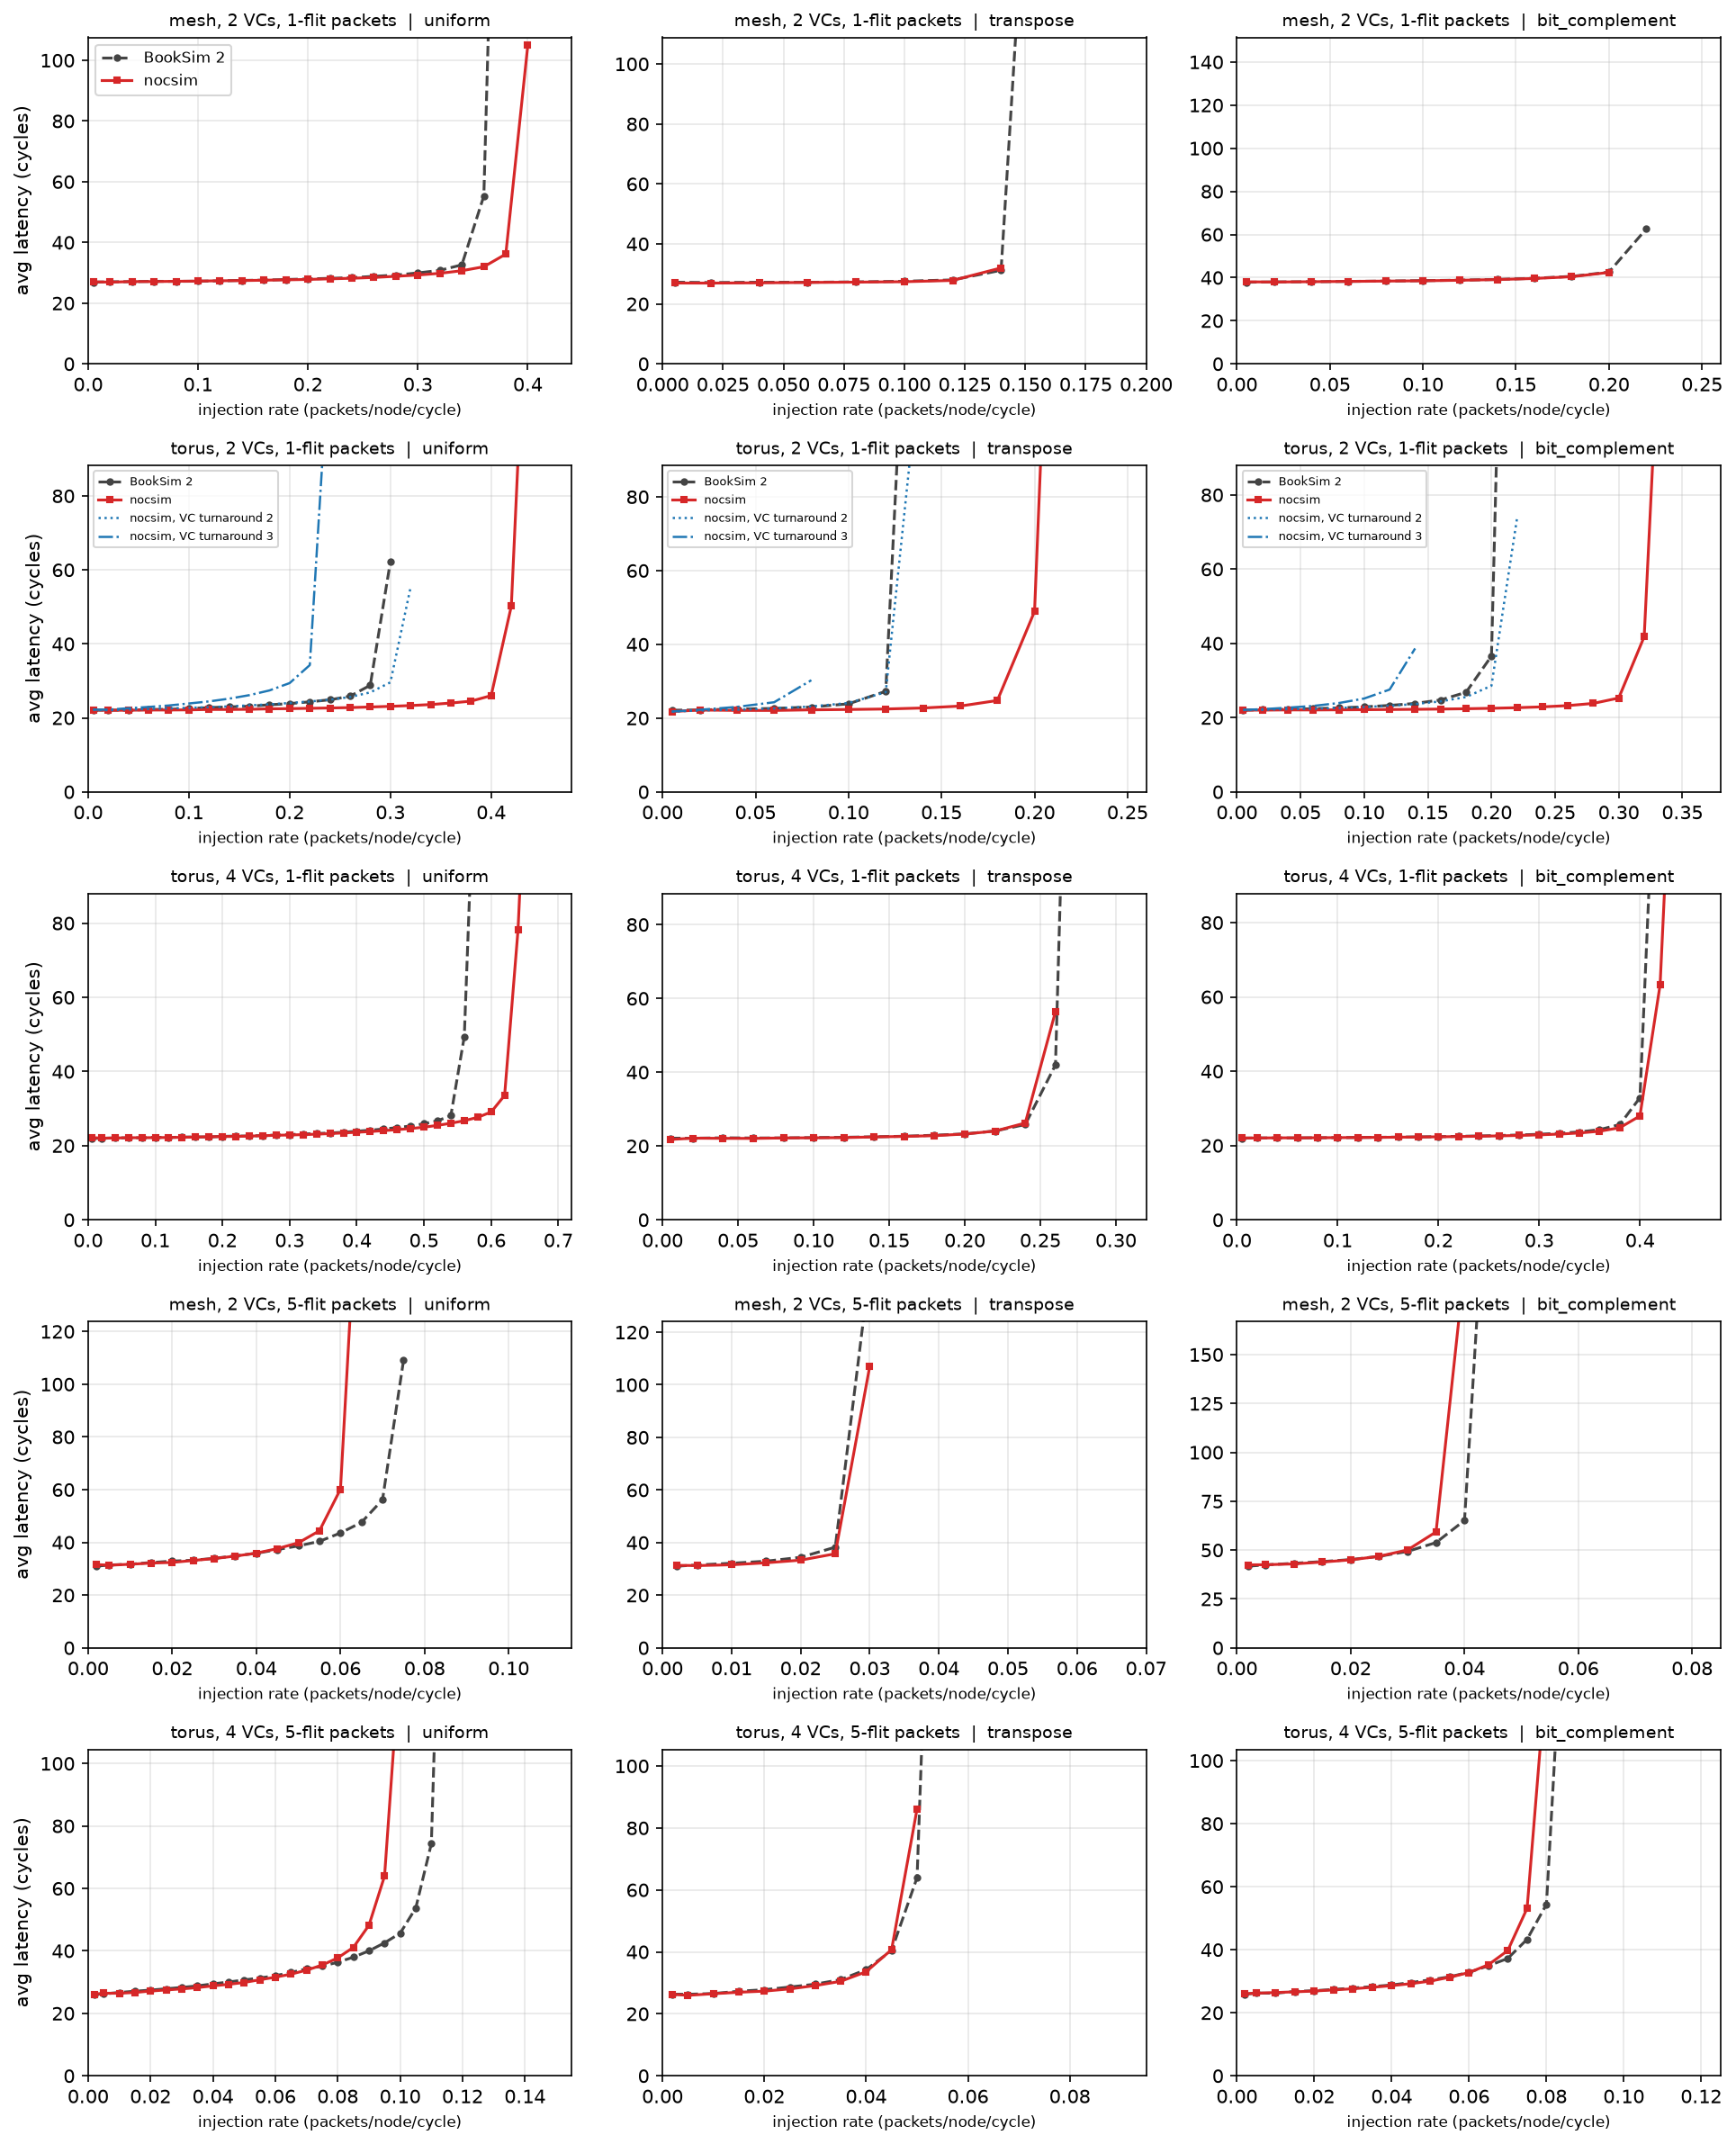
\includegraphics[width=\textwidth]{booksim_validation.png}
  \caption{Our simulator (red) against BookSim~2 (grey, dashed): dimension-order
  routing on $8\times 8$ networks, three seeds per point. Rows: mesh with 2 VCs,
  torus with 2 VCs (one VC per dateline class, with additional curves for a
  2- and 3-cycle VC turnaround), torus with 4 VCs, and 5-flit packets on the
  mesh and 4-VC torus.}
  \label{fig:booksim}
\end{figure}

BookSim cannot run the escape-channel routing, so the validation uses
dimension-order routing, which both simulators implement identically,
including BookSim's dateline VC rule for tori. Router delays are matched
(4 cycles per hop), as are buffer sizes and packet lengths; BookSim's
6-cycle injection/ejection overhead and its self-addressed packets are
corrected for explicitly. Across the mesh, the 4-VC torus and 5-flit packets
(twelve configurations), zero-load latency agrees within 2.1\%, the mean
latency error below saturation is 0.2--5.3\%, and saturation points differ
by at most 0.06 packets/node/cycle (Fig.~\ref{fig:booksim}). On the 2-VC
torus, where each dateline class has a single VC, BookSim saturates much
earlier (0.30 against 0.42 on uniform traffic) because a single VC cannot
forward back-to-back packets through its allocation pipeline. Adding a
2-cycle VC turnaround to our router reproduces BookSim's saturation points
exactly on all three patterns (0.32, 0.12 and 0.20 against 0.30, 0.12 and
0.20). All remaining experiments use this turnaround.

\subsection{Static trade-offs}
\label{sec:res-static}

\begin{table}[t]
\centering
\caption{The six designs at $8\times8$ (1.5~mm tiles, 22~nm). Wire and longest link in tile pitches; throughput estimate averaged over four patterns, relative to the torus; area and wire-limited clock from DSENT.}
\label{tab:designs}
\small
\begin{tabular}{@{}lrrrrrr@{}}
\toprule
Design & Wire & Longest & Hops & Thr. est. & Area (mm$^2$) & Max clock (GHz) \\
\midrule
Mesh                      & 112 & 1 & 5.33 & 0.56 & 15.9 & 4.00 \\
Torus                     & 224 & 7 & 4.06 & 1.00 & 30.0 & 2.45 \\
Folded torus              & 224 & 2 & 4.06 & 1.00 & 29.9 & 4.00 \\
Modified torus            & 176 & 7 & 4.13 & 0.63 & 24.1 & 2.45 \\
Searched (links $\le$ 5)  & 180 & 5 & 3.84 & 0.65 & 24.5 & 3.42 \\
Searched (wire $\le$ 208) & 208 & 9 & 3.79 & 0.71 & 28.0 & 1.86 \\
\bottomrule
\end{tabular}
\end{table}

\begin{figure}[t]
  \centering
  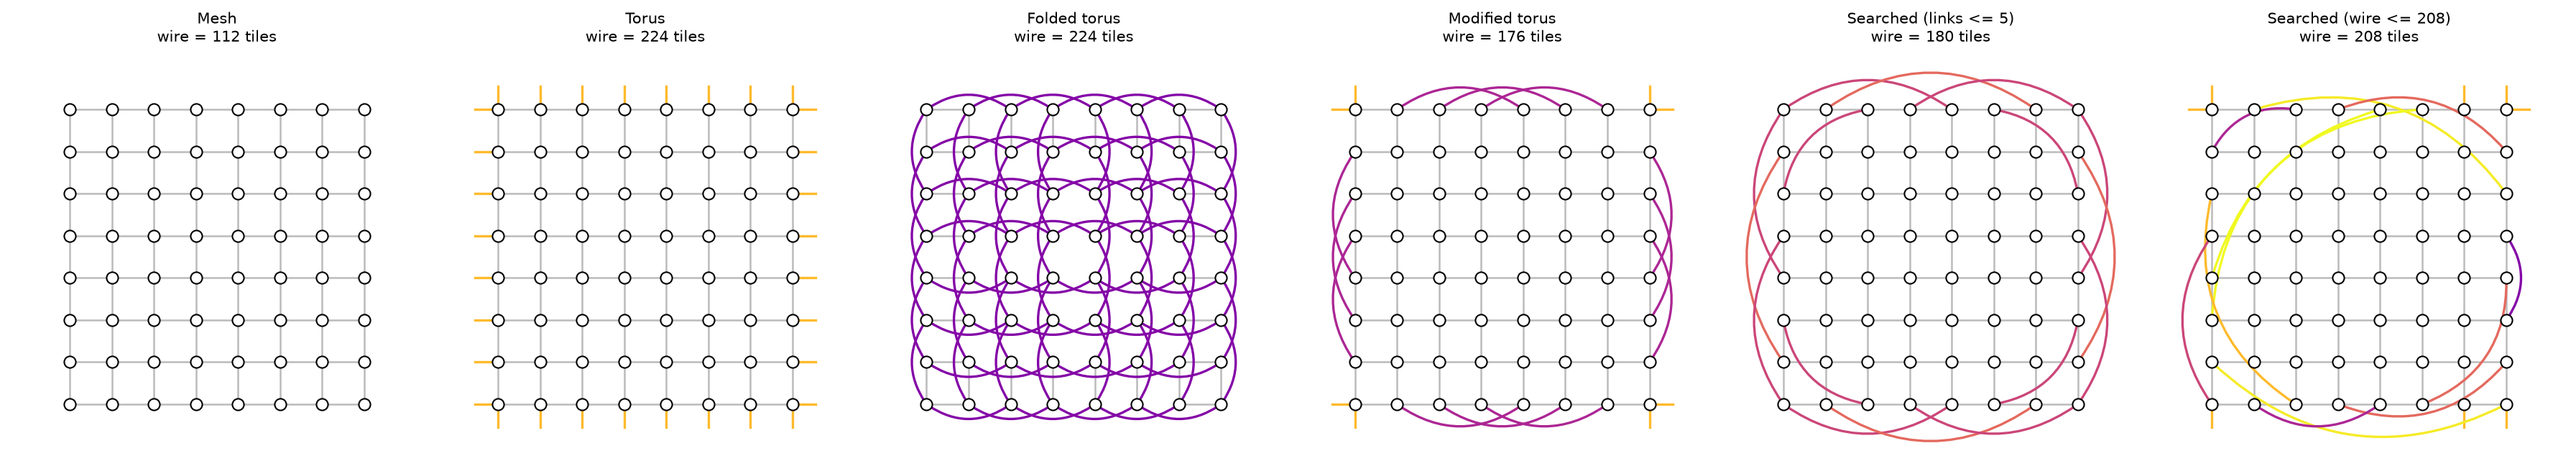
\includegraphics[width=\textwidth]{paper_topologies.png}
  \caption{The six designs. Grey: mesh links. Edge stubs: full-length
  wraparounds. Arcs: other added links, coloured by length.}
  \label{fig:topologies}
\end{figure}

Table~\ref{tab:designs} and Fig.~\ref{fig:topologies} introduce the designs.
The two searched designs come from the two constraint types: the best
design found with a total-wire budget of 208 tiles, and the best found with
no extra link longer than five tiles.

\begin{figure}[t]
  \centering
  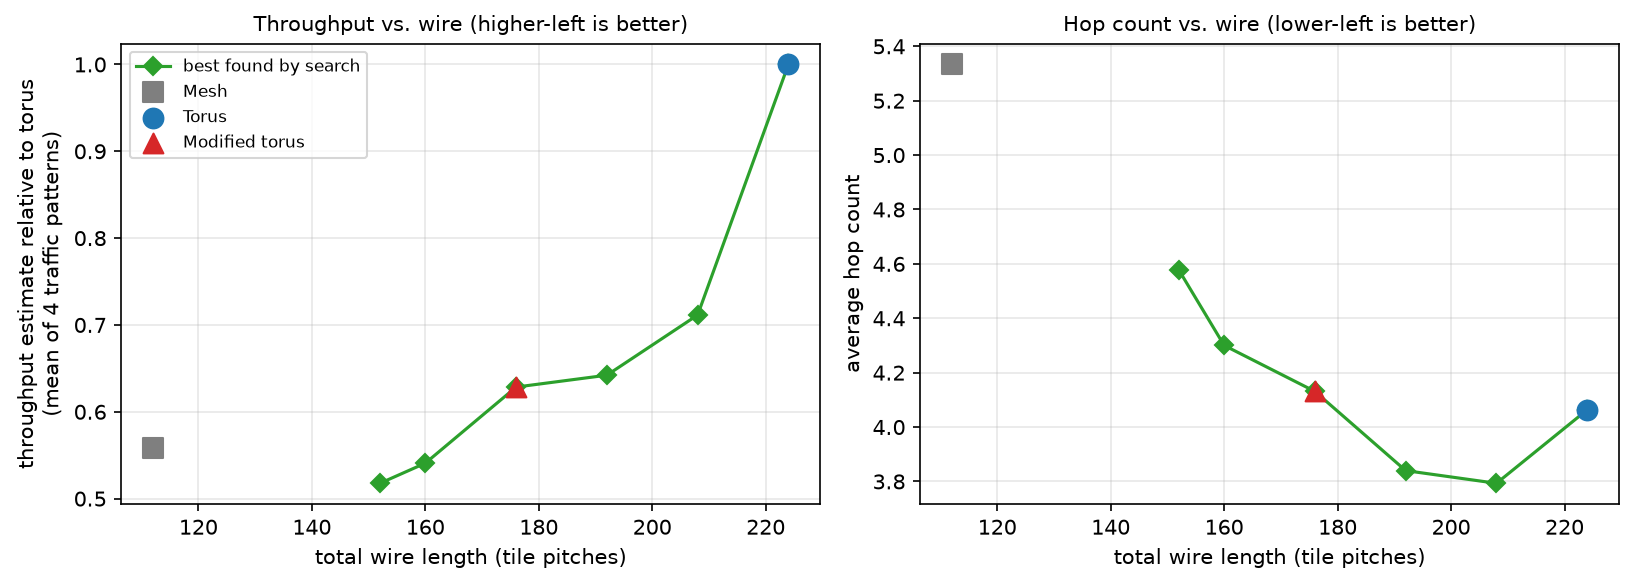
\includegraphics[width=0.49\textwidth]{frontier.png}\hfill
  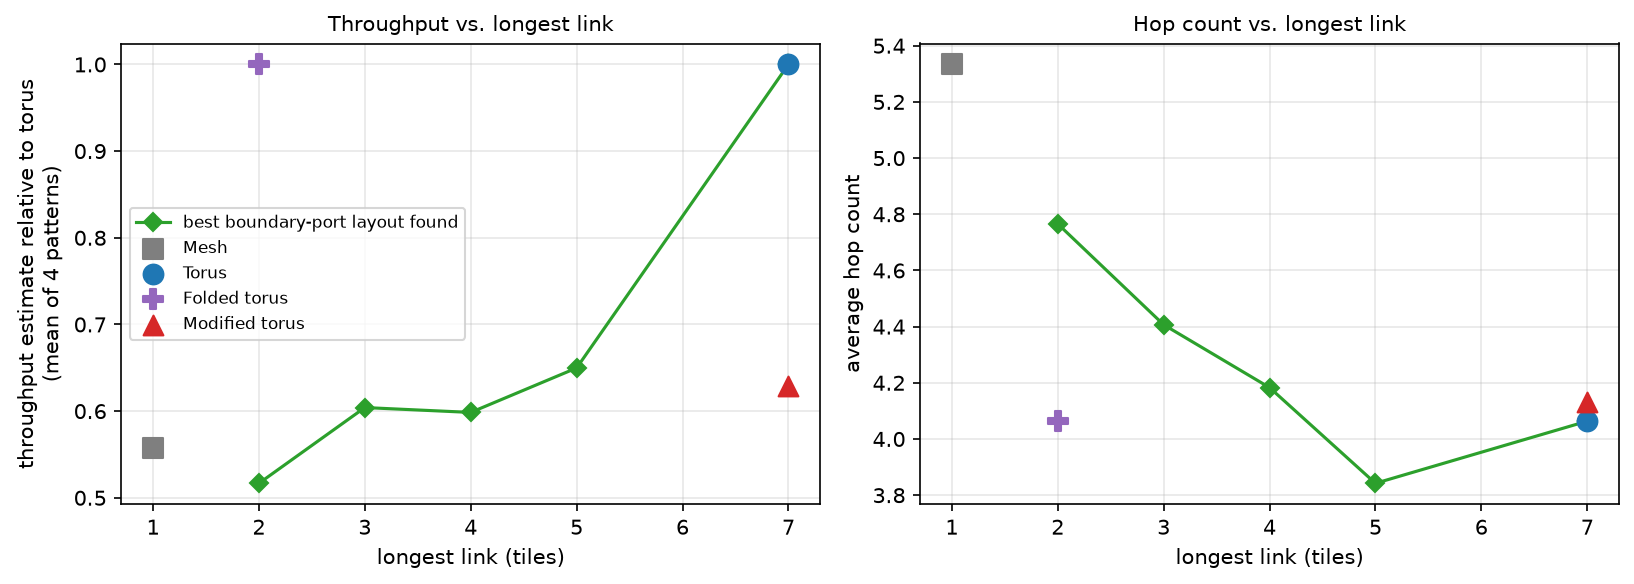
\includegraphics[width=0.49\textwidth]{link_length_search.png}
  \caption{Left: best design found for each total-wire budget. Right: best
  design found for each longest-link limit, against the reference designs.
  Both: throughput estimate relative to the torus (mean of four patterns).}
  \label{fig:frontiers}
\end{figure}

Fig.~\ref{fig:frontiers} shows the two frontiers. Under a total-wire budget
(left), throughput rises slowly from 152 to 208 tiles (0.52 to 0.71 of the
torus) and then jumps to the torus itself at 224 tiles. The modified torus
lies on this frontier: at its 176-tile budget no method found a better
design. Under a longest-link limit (right), the best designs reach 0.52,
0.60 and 0.65 of the torus at limits of 2, 3 and 5 tiles. The folded torus,
outside the space, dominates all of them: the same longest link as the
2-tile designs and the torus's throughput (it is the torus graph with the
same core mapping, so its analytical metrics equal the torus's). Its cost is
wire: 224 tiles against 144--180 for the searched designs. The 5-tile design improves on the modified torus
in hop count (3.84 against 4.13), throughput and longest link (5 against 7
tiles) for 2\% more wire.

\subsection{Area and timing}
\label{sec:res-area}

\begin{figure}[t]
  \centering
  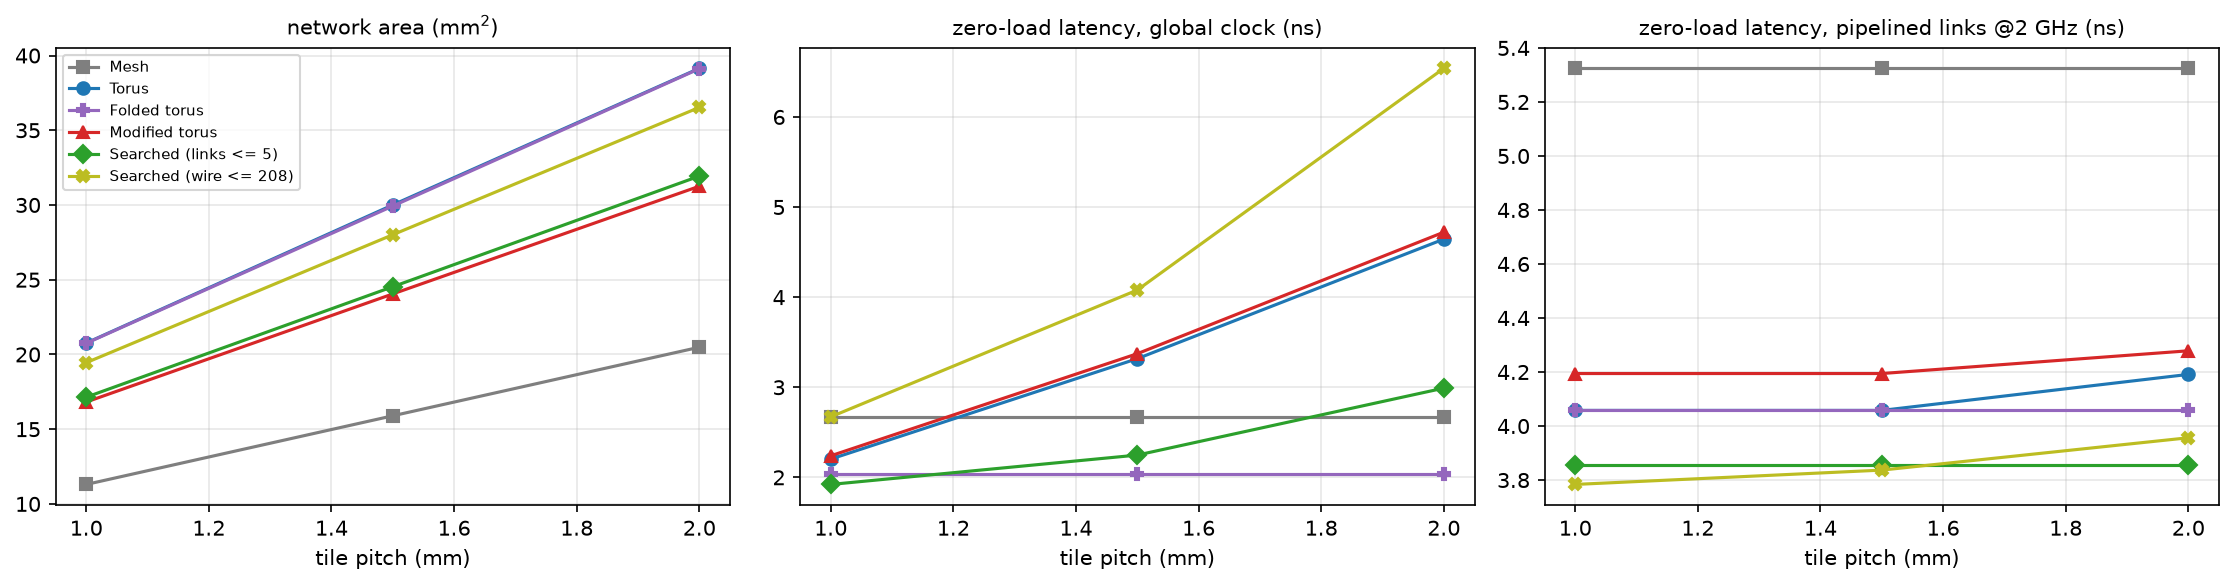
\includegraphics[width=\textwidth]{area_timing.png}
  \caption{Area and zero-load latency against tile pitch (22~nm, DSENT).
  Middle: wire-limited clock. Right: fixed 2~GHz clock.}
  \label{fig:area}
\end{figure}

Wire dominates network area: at 1.5~mm tiles, global-wire tracks are 92\% of
the torus's 30.0~mm$^2$. The modified torus and the 5-tile design save
20\% and 18\% of the torus's area. Under a wire-limited clock, the torus and
modified torus, whose 10.5~mm wraparounds fit in a cycle only up to
2.45~GHz, are slower than the mesh at zero load (3.32 and 3.37~ns, against
2.67~ns), and the 9-tile searched design is slower still (4.08~ns). The folded torus
runs at 4~GHz and is fastest (2.03~ns); the 5-tile design follows
(2.25~ns at 3.42~GHz). At a fixed 2~GHz clock the two searched designs have the lowest zero-load
latencies (3.84 and 3.86~ns, against 4.06~ns for the torus and folded
torus). Fig.~\ref{fig:area} shows that tile pitch shifts these rankings:
at 1~mm the 5-tile design runs at 4~GHz and becomes the fastest network
under a wire-limited clock (1.92~ns), while at 2~mm the wire-limited clocks of the long-link
designs fall to 1.75~GHz (torus, modified torus) and 2.57~GHz (5-tile).

\subsection{Synthetic traffic}
\label{sec:res-synth}
\begin{figure}[t]
  \centering
  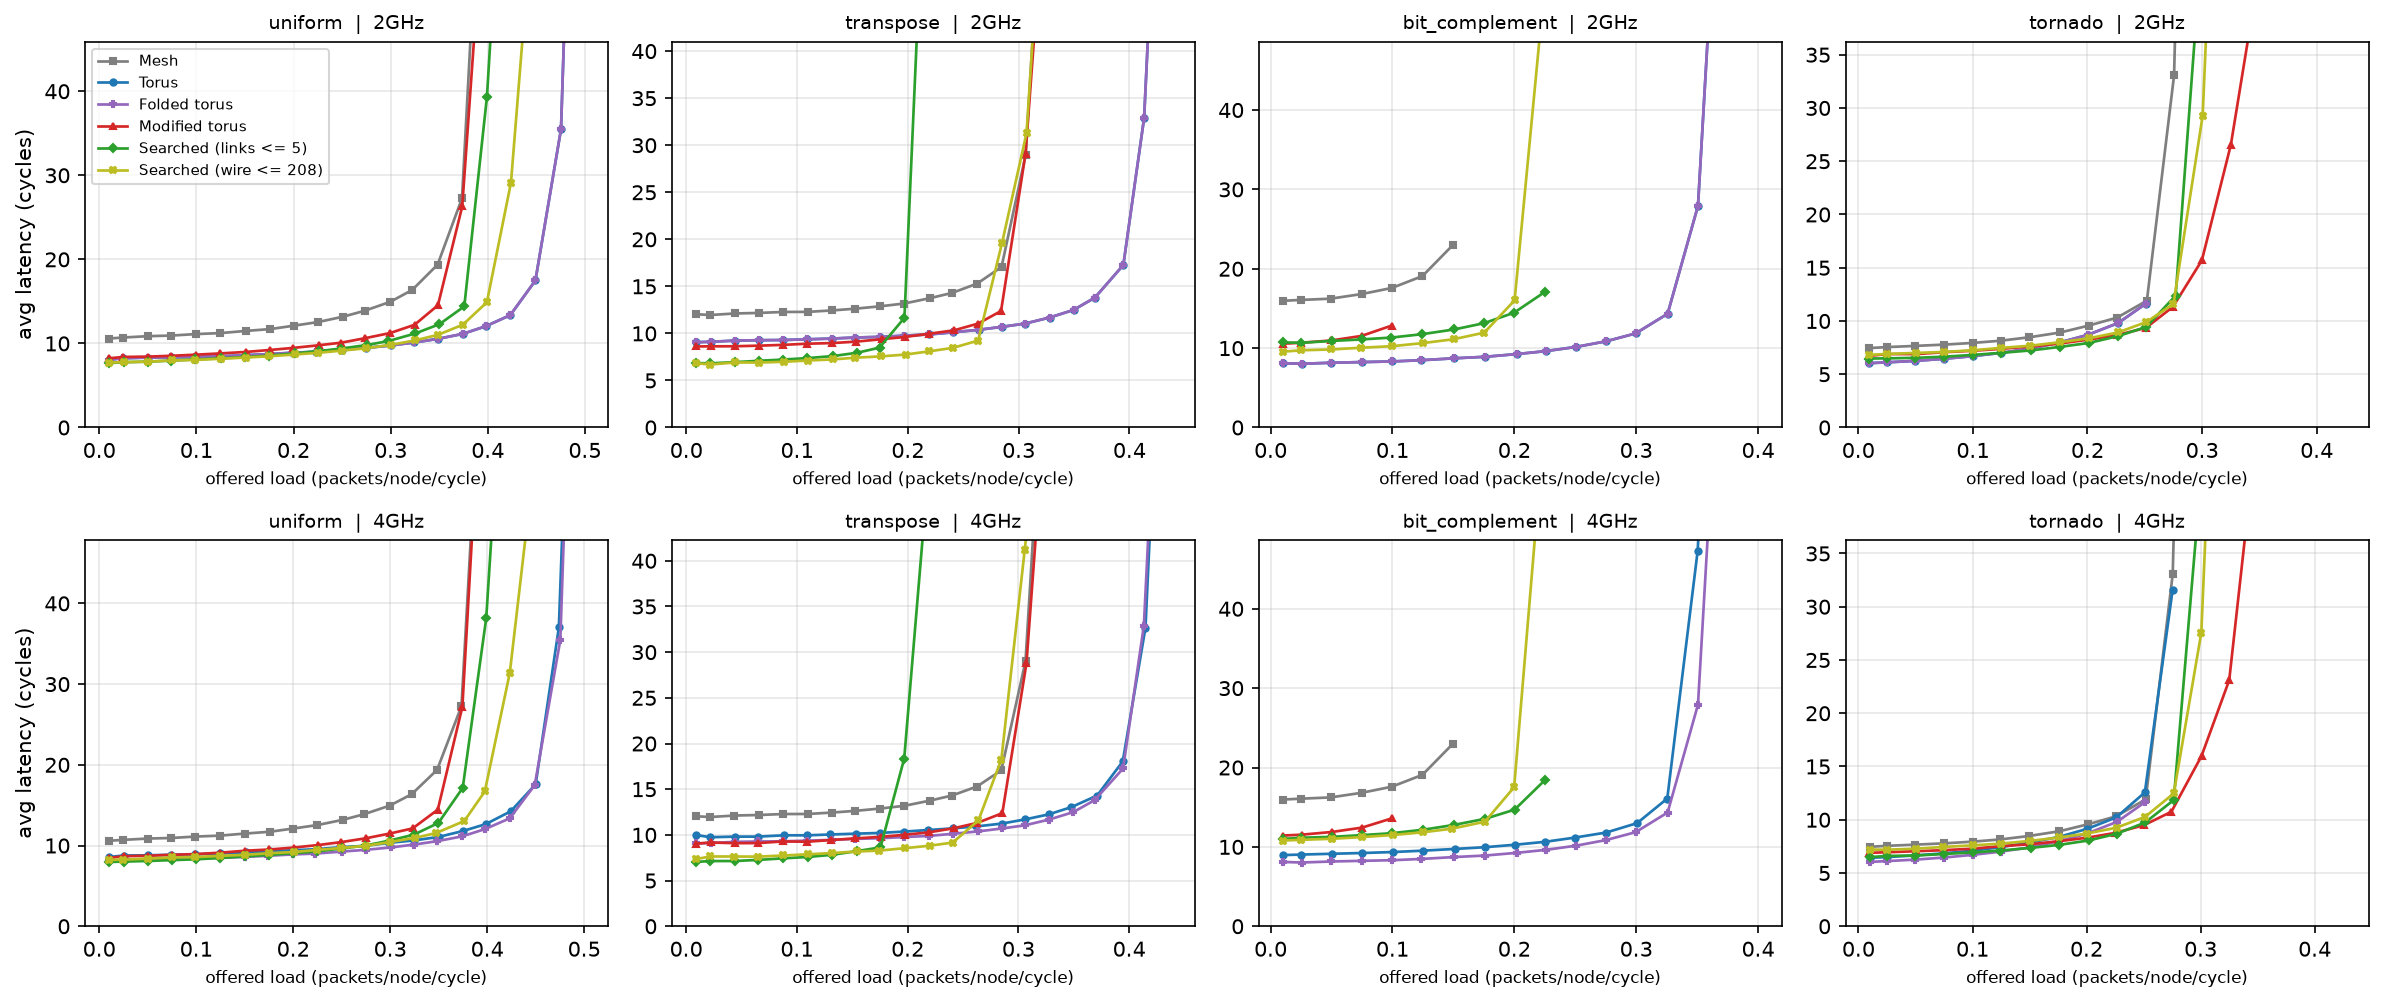
\includegraphics[width=\textwidth]{latency_vs_load.png}
  \caption{Synthetic traffic: average latency (cycles of each clock) against
  offered load. Top row: 2~GHz (all links of the hand designs take one
  cycle). Bottom row: 4~GHz (one cycle reaches 4.3 tiles, so the 7-tile
  wraparounds take two).}
  \label{fig:synth}
\end{figure}

Fig.~\ref{fig:synth} shows load--latency curves under four synthetic
patterns. The searched designs have the lowest zero-load latency on uniform
and transpose traffic (7.65 and 6.85 cycles for the 5-tile design at
2~GHz, against 8.06 and 9.06 for the torus), consistent with their lower hop
counts. Their saturation throughput, however, is not uniformly good. On
uniform traffic the torus and folded torus saturate highest (0.45
packets/node/cycle, against 0.38 for the 5-tile design and the mesh); on
transpose the 5-tile design saturates at 0.20, below the mesh (0.31),
because several transpose flows share its few long links. At 2~GHz the
folded torus behaves exactly like the torus, as it should: same graph, same
traffic, and every link fits in one cycle. The two tori saturate highest on
uniform, transpose and bit-complement traffic; on tornado traffic the
modified torus (0.30) and the 5-tile design (0.28) do better than both tori
(0.25). The modified torus is the weakest long-link design on
bit-complement traffic, saturating at 0.10, below the mesh. At 4~GHz the
two-cycle wraparounds raise the zero-load latency of the torus and modified
torus by 0.2--0.9 cycles, while the folded torus keeps one-cycle links. The application traces run
far below these saturation points even at $50\times$ compression, which is
why the searched designs' latency advantage, rather than their throughput,
determines the application results below.

\subsection{Applications and energy}
\label{sec:res-apps}

\begin{table}[t]
\centering
\caption{PARSEC traces (seven benchmarks, geometric mean), relative to the
mesh; lower is better. EDP: network energy $\times$ runtime.}
\label{tab:apps}
\small
\begin{tabular}{@{}lrrrrrrrr@{}}
\toprule
 & \multicolumn{4}{c}{Fixed 2~GHz clock} & \multicolumn{4}{c}{Wire-limited clock} \\
\cmidrule(lr){2-5}\cmidrule(l){6-9}
 & \multicolumn{2}{c}{$10\times$} & \multicolumn{2}{c}{$50\times$} & \multicolumn{2}{c}{$10\times$} & \multicolumn{2}{c}{$50\times$} \\
Design & Run & EDP & Run & EDP & Run & EDP & Run & EDP \\
\midrule
Torus                     & 0.878 & 0.908 & 0.812 & 0.778 & 1.115 & 1.435 & 1.246 & 1.781 \\
Folded torus              & 0.878 & 0.864 & 0.812 & 0.741 & \textbf{0.909} & \textbf{0.926} & \textbf{0.827} & \textbf{0.771} \\
Modified torus            & 0.872 & 0.863 & 0.803 & 0.734 & 1.108 & 1.366 & 1.233 & 1.682 \\
Searched (links $\le$ 5)  & \textbf{0.826} & \textbf{0.770} & \textbf{0.733} & \textbf{0.608} & 0.923 & 0.955 & 0.852 & 0.816 \\
Searched (wire $\le$ 208) & 0.829 & 0.796 & 0.738 & 0.633 & 1.202 & 1.628 & 1.425 & 2.269 \\
\bottomrule
\end{tabular}
\end{table}

\begin{figure}[t]
  \centering
  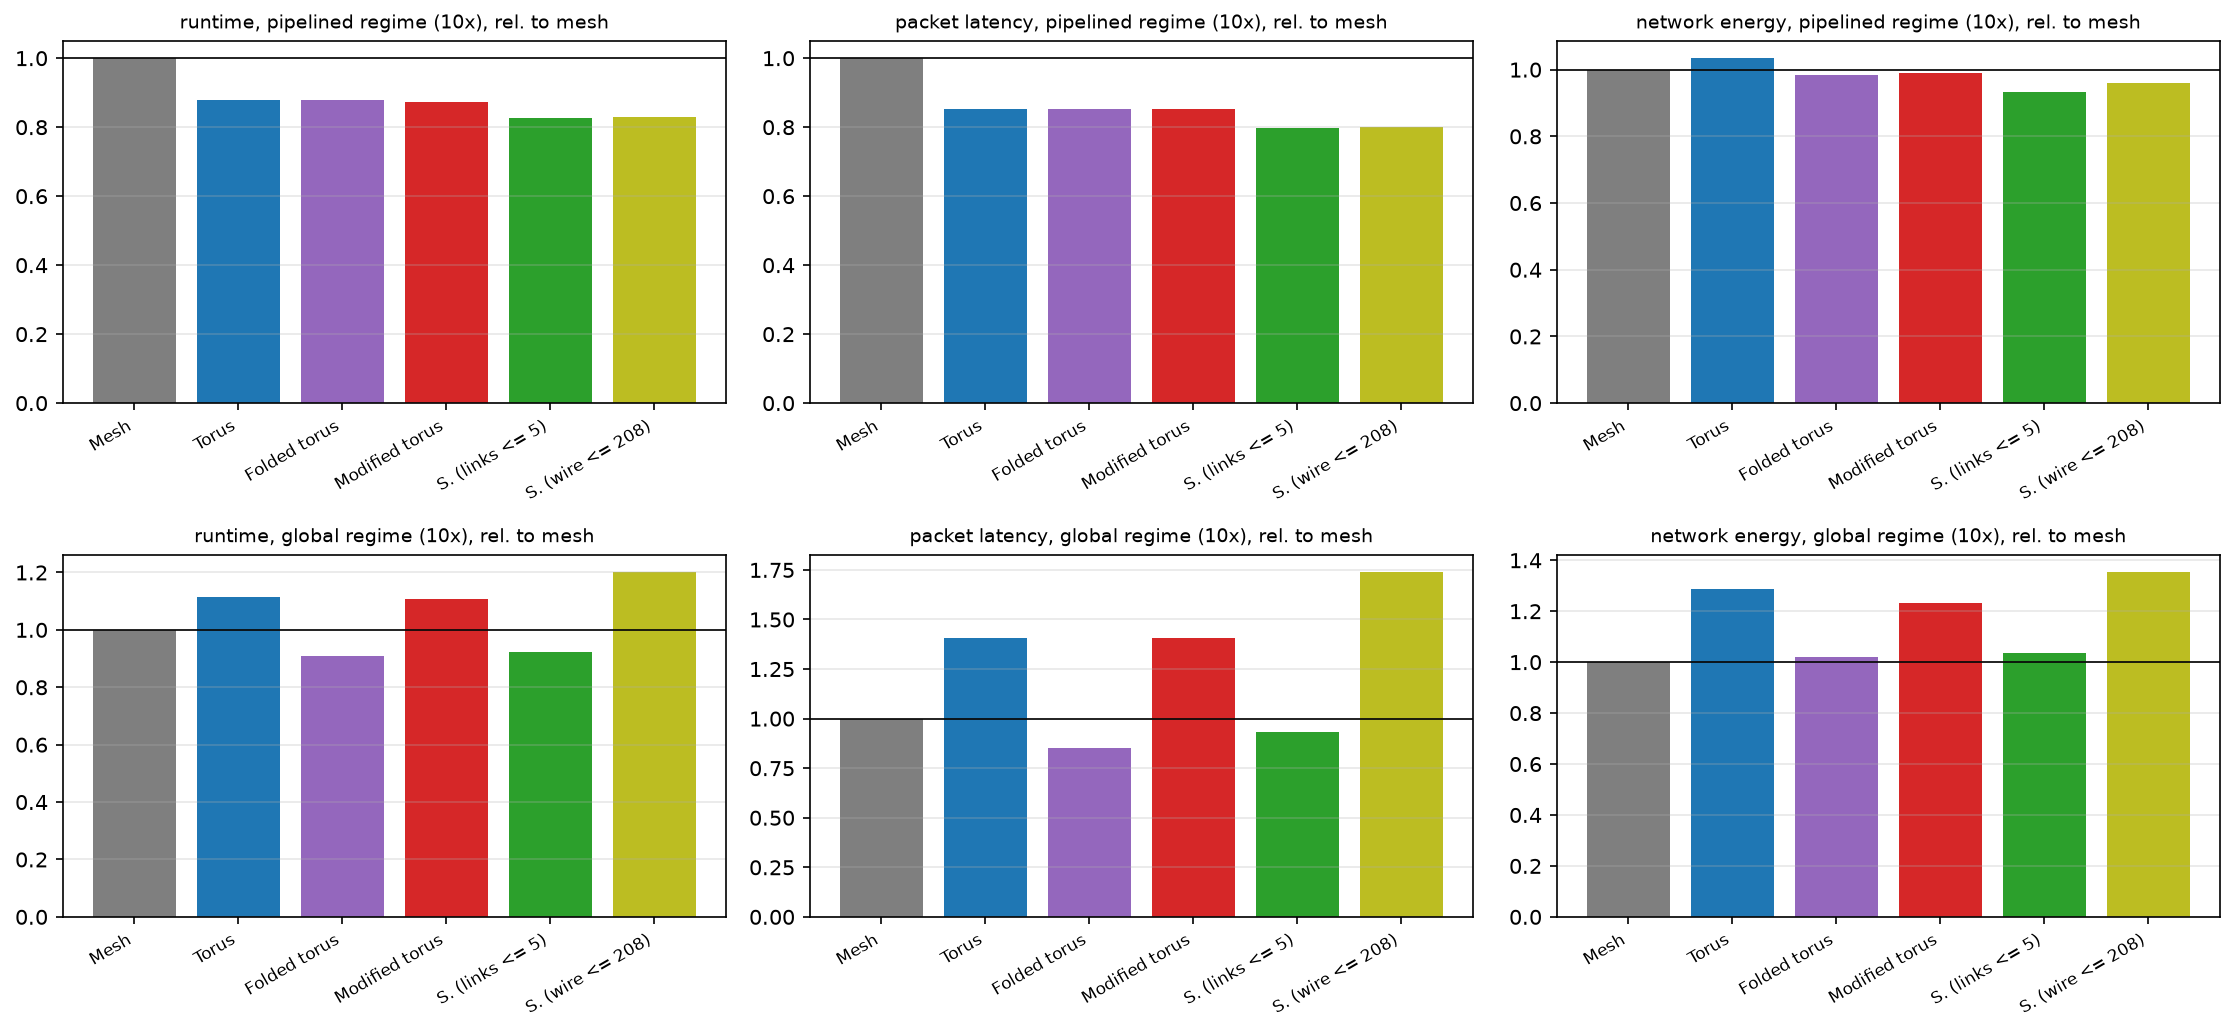
\includegraphics[width=\textwidth]{applications.png}
  \caption{PARSEC traces at $10\times$ compression, relative to the mesh
  (geometric mean of seven benchmarks). Top: fixed 2~GHz clock. Bottom:
  wire-limited clock.}
  \label{fig:apps}
\end{figure}

All 252 trace runs completed without deadlock. At the recorded speed
($1\times$), every design finishes within 1.1\% of the mesh: at the load of
these traces the network is rarely on the critical path, and because every
radix-4 design has more router ports than the mesh's edge routers and more
link repeaters, all of them consume 11--17\% \emph{more} network energy than
the mesh. The comparison of the long-link designs becomes meaningful under
compression (Table~\ref{tab:apps}, Fig.~\ref{fig:apps}).
Table~\ref{tab:perbench} breaks the $10\times$ results down by benchmark:
the rankings below hold on six of the seven benchmarks, and the seventh
(vips) is insensitive to the network, with every design within 0.1\% of the
mesh.

\emph{At a fixed clock}, the 5-tile searched design is the best evaluated
network at both compression levels: at $50\times$ it runs 10\% faster than
the torus and folded torus (which behave identically at this clock) and 9\%
faster than the modified torus, and has the lowest energy-delay product
(0.608 of the mesh). Network energy is dominated by leakage and clock power,
so it follows runtime; dynamic energy alone is lowest on the mesh and 2\%,
4\%, 7\% and 8\% higher on the 5-tile design, modified torus, folded torus
and torus respectively.

\emph{With a wire-limited clock}, the folded torus is the best evaluated
design (runtime 0.827 and EDP 0.771 of the mesh at $50\times$). The torus
and modified torus, held to 2.45~GHz by their wraparounds, run 23--25\%
\emph{slower} than the mesh, and the 9-tile searched design is worse still.
The 5-tile design is second, 1.5\% behind the folded torus at $10\times$ and
3\% at $50\times$, with 18\% less area.

\emph{Tile pitch.} Repeating the $10\times$ runs at 1.0 and 2.0~mm tiles
confirms the static picture. At 1.0~mm the 5-tile design is the best
or tied-best evaluated design in both regimes (wire-limited runtime 0.870 and EDP 0.847,
against 0.909 and 0.925 for the folded torus). At
2.0~mm, under a wire-limited clock, the folded torus is the only design
that beats the mesh, and the 5-tile design falls behind it (runtime
1.035). At a fixed clock the 5-tile design has the lowest runtime at every
pitch (tied within 0.1\% with the 208-tile design at 1.0~mm).

\emph{Escape-channel rule.} Rerunning the $10\times$ and $50\times$
experiments with packets confined to the escape channel once they enter it
changes runtime and energy by at most 0.2\% for every design and regime, so
the results do not depend on letting packets return to adaptive channels.

\begin{table}[t]
\centering
\caption{Runtime relative to the mesh for each PARSEC benchmark ($10\times$ compression, 1.5~mm tiles); lower is better. Best evaluated design per row in bold.}
\label{tab:perbench}
\small
\begin{tabular}{@{}lrrrrrrrrrr@{}}
\toprule
 & \multicolumn{5}{c}{Fixed 2~GHz clock} & \multicolumn{5}{c}{Wire-limited clock} \\
\cmidrule(lr){2-6}\cmidrule(l){7-11}
Benchmark & Torus & Folded & Modified & S.\,$\le$5 & S.\,$\le$208 & Torus & Folded & Modified & S.\,$\le$5 & S.\,$\le$208 \\
\midrule
blackscholes & 0.811 & 0.811 & 0.801 & \textbf{0.745} & 0.749 & 1.139 & \textbf{0.848} & 1.125 & 0.867 & 1.268 \\
canneal & 0.859 & 0.859 & 0.854 & \textbf{0.806} & 0.808 & 1.134 & \textbf{0.896} & 1.129 & 0.918 & 1.245 \\
ferret & 0.895 & 0.895 & 0.891 & \textbf{0.844} & 0.849 & 1.114 & \textbf{0.928} & 1.110 & 0.941 & 1.197 \\
fluidanimate & 0.878 & 0.878 & 0.871 & \textbf{0.822} & 0.824 & 1.118 & \textbf{0.914} & 1.110 & 0.926 & 1.198 \\
swaptions & 0.848 & 0.848 & 0.851 & \textbf{0.795} & 0.800 & 1.146 & \textbf{0.883} & 1.150 & 0.911 & 1.275 \\
vips & 0.999 & 0.999 & 0.999 & 0.999 & \textbf{0.999} & 1.000 & \textbf{1.000} & 1.000 & 1.000 & 1.001 \\
x264 & 0.866 & 0.866 & 0.848 & \textbf{0.790} & 0.794 & 1.160 & \textbf{0.899} & 1.137 & 0.905 & 1.255 \\
\midrule
Geo.\ mean & 0.878 & 0.878 & 0.872 & 0.826 & 0.829 & 1.115 & 0.909 & 1.108 & 0.923 & 1.202 \\
\bottomrule
\end{tabular}
\end{table}


\subsection{Search methods (secondary)}
\label{sec:res-search}

\begin{table}[t]
\centering
\caption{Search at the modified torus's 176-tile budget: 2500 objective
evaluations, three seeds. Throughput relative to the torus.}
\label{tab:search}
\small
\begin{tabular}{@{}lrrr@{}}
\toprule
Method & $J$ (mean $\pm$ std) & Thr. & Hops \\
\midrule
Random search        & $-0.03 \pm 0.08$ & 0.42 & 3.92 \\
REINFORCE            & $0.25 \pm 0.03$  & 0.50 & 4.10 \\
Simulated annealing  & $0.34 \pm 0.02$  & 0.59 & 4.04 \\
Modified torus       & $0.37$           & 0.63 & 4.13 \\
\bottomrule
\end{tabular}
\end{table}

Table~\ref{tab:search} compares the search methods at equal evaluation
budgets. Annealing from random starts comes within 0.03 of the modified
torus; annealing started from it finds nothing better, so the hand design
is (empirically) locally optimal at its budget, much as NetSmith found
Kite-Small optimal for one of its objectives \cite{netsmith}. REINFORCE,
with a tabular autoregressive policy that picks a partner for each port,
lies between random search and annealing. Its policy has a separate logit
for every port pair and no notion of geometry, so it cannot generalise from
one pairing to a similar one; a policy that shares parameters across
positions, such as a graph neural network, is the natural next step, and
learned performance models \cite{noception,noctopus} could replace the
analytical proxy inside the search. Each annealing run takes a few minutes
for 64 routers, against the multi-day MILP solves NetSmith reports for 48
\cite{netsmith}, at the price of no optimality guarantee.

% ===========================================================================
\section{Discussion}
\label{sec:discussion}

\paragraph{Which design to use} The results separate the two wire costs.
If the clock is set by the longest wire, length is what matters and,
among the evaluated designs, the folded torus wins: it has the torus's graph, links of at most two tiles,
and the best performance at 1.5--2~mm pitches, at the cost of the most
wire. If links can be pipelined or the clock is set elsewhere, a searched
design that keeps links moderately long (at most five tiles) and saves
18\% of the torus's area is the fastest evaluated network. Designs that save total
wire but keep a few full-length links, including the modified torus, give
up most of the torus's advantage in exchange for area: they are never the
best choice on performance.

\paragraph{Threats to validity}
\begin{itemize}
\item \emph{Traces.} Netrace's traces come from in-order cores and are
  light; the network barely affects runtime at recorded speed. Compression
  emulates faster cores but not a different memory system. Full-system
  simulation, as in NetSmith, would be stronger.
\item \emph{Physical model.} Areas and energies come from DSENT models, not
  layout; wire length is the Manhattan distance between tiles (or the
  folded layout's length for the folded torus); DSENT's 22, 32 and 45~nm
  models share global-wire dimensions.
\item \emph{Simulator.} Virtual cut-through rather than wormhole and a
  greedy separable allocator. The validation against BookSim covers
  dimension-order routing only, as BookSim cannot run the escape scheme.
\item \emph{Scope.} One grid size ($8\times 8$), radix 4, boundary-port
  designs only; the folded torus shows that rewiring interior links can do
  better, which this space excludes by construction. We do not compare
  against a topology generated by NetSmith or the Library of Networks: both
  target concentrated interposer networks with a different router layout
  and radix, NetSmith relies on a commercial MILP solver, and at 64 routers
  its reported solve times run to days; a like-for-like comparison would
  need its formulation re-targeted to monolithic radix-4 grids.
\item \emph{Folded-torus mapping.} If cores instead keep their tile
  positions and only the wiring is folded, physically defined permutation
  patterns map onto different flows and the folded torus's analytical
  throughput rises to 1.26 of the flat torus; we use the same-mapping
  comparison throughout.
\end{itemize}

% ===========================================================================
\section{Conclusion}
\label{sec:conclusion}

Pairing a mesh's spare boundary ports is a small, floorplan-compatible
design space that already contains the torus and edge-folded designs. Our
evaluation, grounded in a BookSim-validated simulator, PARSEC traces and
DSENT, shows that the right design depends on which wire cost dominates.
When the longest wire sets the clock, the folded torus is the best of the
evaluated designs. At a fixed
clock, a searched design whose extra links are at most five tiles long
reduces runtime by 17\% and energy-delay product by 23\% against a mesh
under compressed traffic, outperforms the torus and folded torus, and needs
20\% less wire than a torus. Saving
total wire while keeping full-length links, the idea behind the design
this study started from, buys area but not performance.

% ===========================================================================
\section*{Data availability}
The simulator, analysis code, trace-conversion and DSENT drivers, searched
designs and all raw results are available at
\url{https://github.com/R4hulR/nocsim}. The Netrace traces are available
from their authors \cite{netrace}.

\section*{CRediT authorship contribution statement}
\textbf{Rahul Ray:} Conceptualization, Methodology, Software, Validation,
Formal analysis, Investigation, Data curation, Writing -- original draft,
Writing -- review \& editing, Visualization.

\section*{Declaration of competing interest}
The author declares that they have no known competing financial interests
or personal relationships that could have appeared to influence the work
reported in this paper.

\section*{Acknowledgements}
The modified torus topology was first proposed in a B.Tech.\ thesis at
Assam University with S.~Sharma and B.~R.~S.~Satyanarayana, supervised by
Dr.~A.~Biswas \cite{thesis2023}. This research did not receive any specific
grant from funding agencies in the public, commercial, or not-for-profit
sectors.

\bibliographystyle{elsarticle-num}
\bibliography{references}

\end{document}
